\pagenumbering{gobble}
	\underline{\textbf{User interface design}}
	\begin{legal}
	\item \textbf{UX Diagram}
	\begin{center}
		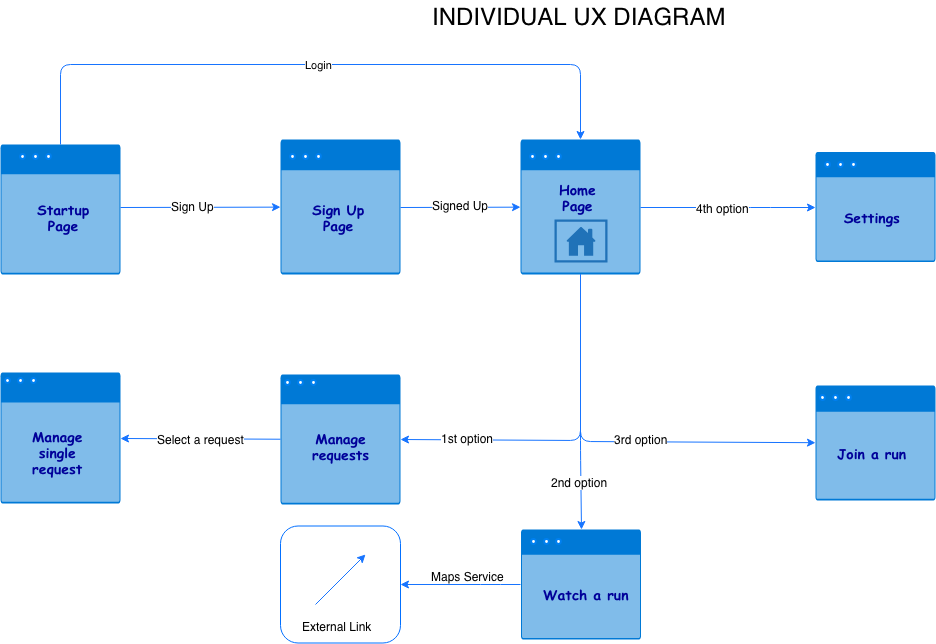
\includegraphics[width=16cm]{../images/design/IndividualUX.png}
	\end{center}
	\begin{center}
		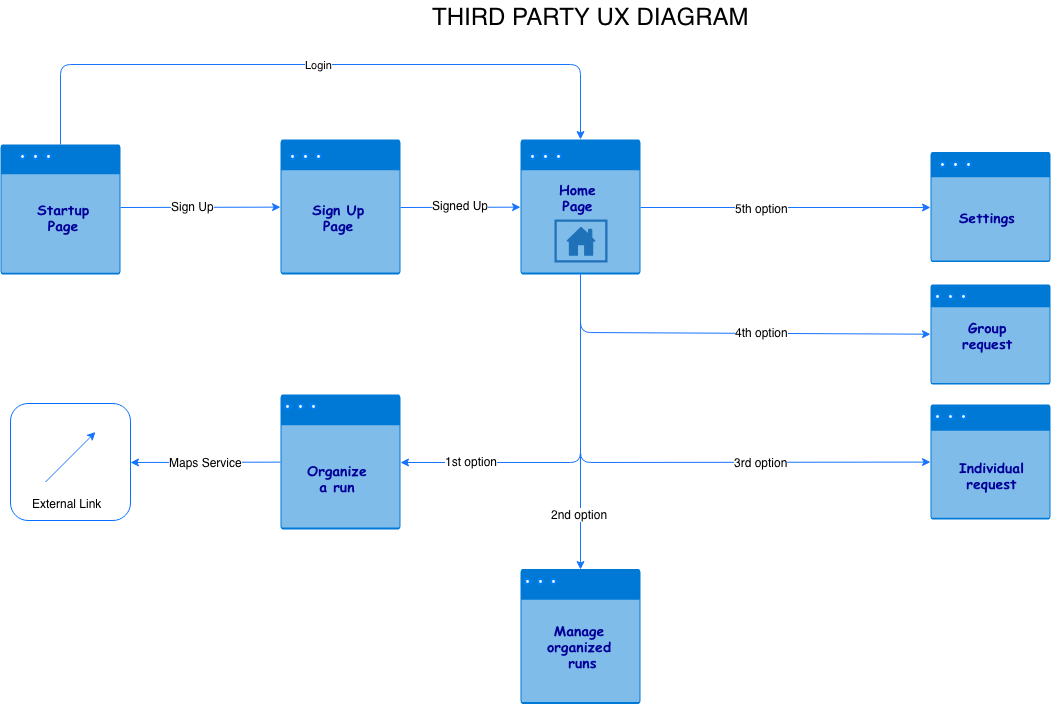
\includegraphics[width=16cm]{../images/design/ThirdPartyUX.png}
	\end{center}
	\end{legal}
\newpage
For the user interface design, we refer to section 3.1.1 of the RASD document. This section is aimed to enrich what was shown in the RASD through two User Experience diagrams. Their main goal is to explain as clear as possible the relationships between the various sections of the application (addressed to the Individuals) and the various pages of the website (addressed to the Third parties).\\
The two diagrams logically share the operations that allow the client to log into the application: 
	\begin{itemize}
	\item Startup Page;
	\item Login;
	\item Sign Up.
	\end{itemize}
Anyway, their presentation will be different due to the Mobile configuration for the Individuals and the Web based configuration for the Third Parties.
The two diagrams start diverging from the principal window of the application/website, that is the Home Page.
In the Individual UX Diagram, it is shown that through the Home Page the user can choose different options:
	\begin{itemize}
	\item Join a run, that allows the user to visualize the available races and select the one he wants to join;
	\item Manage requests, that allows the user to accept/refuse the pending requests coming from the Third parties or visualize/modify the already accepted requests;
	\item Open settings, that allows the user to modify his/her password, personal info, manage the connection between the smartphone and the smartwatch (or a similar device) or enable/disable the AutomatedSOS service.\\ 
	\end{itemize}
In the Third Party UX Diagram, the Home Page is essentially different from the other one and it allows the third party to choose the following options:
	\begin{itemize}
	\item Organize a run, that allows the third party to select che date, time and place of the event. Moreover, it is possible to select the race track thanks to the use of the Maps external service;
	\item Manage runs, whose goal is to allow a third party to visualize and check/modify the status of the runs organized by itself;
	\item Send an Individual request, through which the third party can directly ask a user for his health data, or subscribe to them;
	\item Send a Group request, through which the third party can ask the TrackMe system for aggregated data regarding more than 1000 users grouped by age and residence;
	\item Open settings, that allows the Third party to modify its password.\\
	\end{itemize}

